\documentclass{article}
\usepackage{tikz}
\usetikzlibrary{arrows.meta,positioning,calc,shapes.geometric}
\pagestyle{empty}
\begin{document}
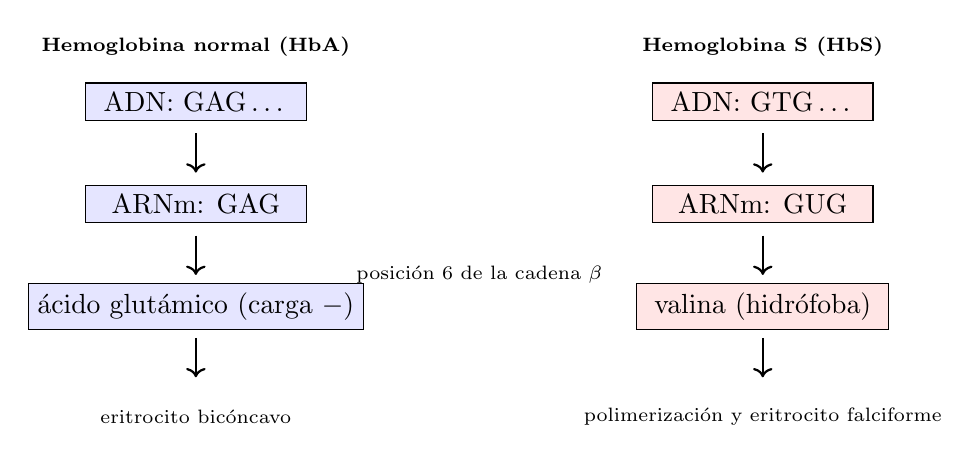
\begin{tikzpicture}

\node[font=\bfseries\scriptsize] at (0,3.2) {Hemoglobina normal (HbA)}; \node[font=\bfseries\scriptsize] at (7.2,3.2) {Hemoglobina S (HbS)};
\node[draw, fill=blue!10, minimum width=2.8cm] at (0,2.5) {ADN: GAG\,\ldots}; \node[draw, fill=red!10, minimum width=2.8cm] at (7.2,2.5) {ADN: GTG\,\ldots};
\draw[->, thick] (0,2.1) -- (0,1.6); \draw[->, thick] (7.2,2.1) -- (7.2,1.6);
\node[draw, fill=blue!10, minimum width=2.8cm] at (0,1.2) {ARNm: GAG}; \node[draw, fill=red!10, minimum width=2.8cm] at (7.2,1.2) {ARNm: GUG};
\draw[->, thick] (0,0.8) -- (0,0.3); \draw[->, thick] (7.2,0.8) -- (7.2,0.3);
\node[draw, fill=blue!10, minimum width=3.2cm] at (0,-0.1) {ácido glutámico (carga $-$)}; \node[draw, fill=red!10, minimum width=3.2cm] at (7.2,-0.1) {valina (hidrófoba)};
\draw[->, thick] (0,-0.5) -- (0,-1.0); \draw[->, thick] (7.2,-0.5) -- (7.2,-1.0);
\node[font=\scriptsize, align=center] at (0,-1.5) {eritrocito bicóncavo}; \node[font=\scriptsize, align=center] at (7.2,-1.5) {polimerización y eritrocito falciforme};
\node[font=\scriptsize] at (3.6,0.3) {posición 6 de la cadena $\beta$};

\end{tikzpicture}
\end{document}
